
\section{Carrier--Greenspan transient solution}

A transient solution for flows on a sloping beach was proposed by Carrier and Greenspan~\cite{CG1958}. The water moves to the shore at an early time, then it becomes still when time is large.

Consider the dimensionless shallow water equations, as presented in the Carrier--Greenspan periodic solution.

The analytical solution is:
\begin{equation}
w = - \frac{u^2}{2} + \epsilon {Re} 
\left[1- 2 \frac{5/4 - i\lambda}{\left\{(1-i\lambda)^2 + \sigma^2 \right\}^{3/2}}
+ \frac32 \frac{(1-i\lambda)^2}{\left\{ (1-i\lambda)^2 + \sigma^2 \right\}^{5/2}} \right],
\end{equation}
\begin{equation}
u = \frac{8\epsilon}{a} {Im} \left[ \frac{1}{\left\{(1-i\lambda)^2 + \sigma^2 \right\}^{3/2}}
- \frac34 \frac{1-i\lambda}{\left\{ (1-i\lambda)^2 + \sigma^2 \right\}^{5/2}}    \right],
\end{equation}
where
\begin{equation}
t = \frac12 a\lambda -u\,, \quad c = \frac14 a\sigma\,,
\end{equation}
in which $c=\sqrt{gh}$ is the wave propagation speed.
Here $\sigma \geq 0$ and we take $a=1.5(1+0.9\epsilon)^{1/2}$. Carrier and Greenspan~\cite{CG1958} observed that the waves do not break if $\epsilon$ is very small, namely $\epsilon \leq 0.23$. Setting $\sigma=0$ into this solution, we get the motion of the shoreline.

The initial condition is given by setting time $t=0$ in this analytical solution. Note that this analytical solution is defined in the dimensionless space. To implement this in the numerical test, we just need to scale it back to the dimensional space.

\subsection{Results}

We consider $\epsilon=0.2$. The following three figures show the stage, $x$-momentum, and $y$-momentum at several instants in time. We should see excellent agreement between the analytical and numerical solutions.

\begin{figure}
\begin{center}
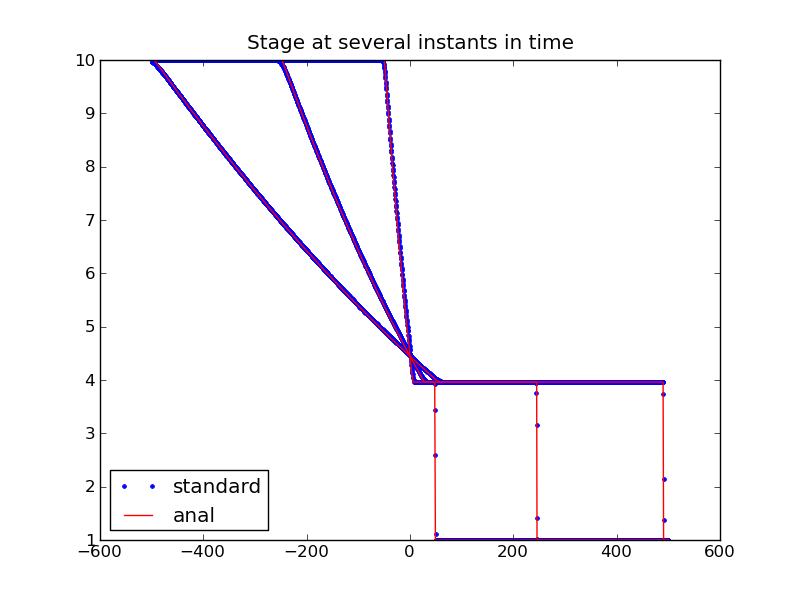
\includegraphics[width=0.9\textwidth]{stage_plot.png}
\end{center}
\caption{Stage results}
\end{figure}

\begin{figure}
\begin{center}
\includegraphics[width=0.9\textwidth]{xmom_plot.png}
\end{center}
\caption{Xmomentum results}
\end{figure}

\begin{figure}
\begin{center}
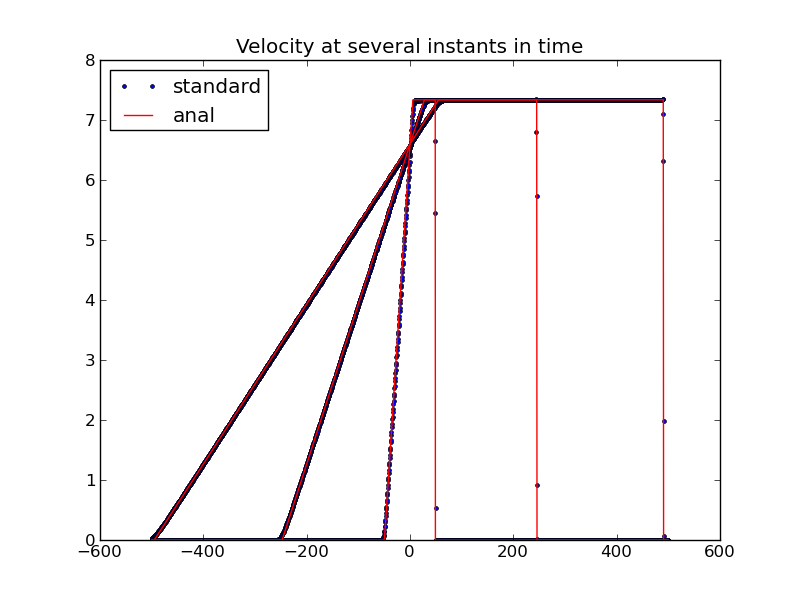
\includegraphics[width=0.9\textwidth]{xvel_plot.png}
\end{center}
\caption{Xvelocity results}
\end{figure}

\endinput
